\chapter{Цели и задачи работы}
\textbf{Цель работы} --- приобрести навыки использования списков и стандартных функций Lisp.
\textbf{Задачи работы} --- изучить способ использования списков для фиксации информации, внутреннее представление одноуровневых и структурированных списков, методы их обработки с использованием базовых функций Lisp.
\chapter{Теоретические вопросы}
\section{Элементы языка: определение, синтаксис, представление в памяти}
Атом --- элементарные данные. Атомами являются:
\begin{itemize}
\item символы (идентификаторы) --- набор литер (литера --- буква или цифра), начинающихся с буквы;
\item специальные символы --- T и Nil;
\item самоопределяемые атомы --- натуральные числа, дробные числа, вещественные числа, строки (последовательность символов, заключённая в двойные апрстрофы).
\end{itemize}

Точечная пара --- единая универсальная базовая структура для конструирования сложных символьных выражений. Представляет из себя сложную структуру, состоящую из двух атомов. В памяти представляется бинарным узлом, левая и правая части которого равноправны и хранят указатели на эти атомы. Вместо атомов могут быть использованы более сложные выражения.
Точечная пара ::= (<атом>.<атом>) | (<атом>.<точечная пара>) | (<точечная пара>.<атом>) | (<точечная пара>.<точечная пара>)\\

S-выражение (символьное выражение) - это или атом или заключённая в скобки пара из двух S-выражений, разделённых точкой. Все сложные символьные выражения являются S-выражениями, а в памяти представляются структурами из одинаково устроенных блоков - бинарных узлов, содержащих указатели на S-выражения. Каждый бинарный узел соответствует минимальному блоку памяти из двух указателей.

S-выражение ::= <атом>|<точечная пара>\\

Список --- рекурсивная структура, которая может быть описана следующими БНФ (формулами Бэкуса-Наура):

список ::= ( последовательность\_элементов ) | пустой список

последовательность\_элементов ::= элемент | элемент  последовательность\_элементов

элемент ::= атом | список

пустой список ::= () | NIL

Пробелы используются в качестве разделителей элементов списка.

\section{Особенности языка Lisp. Структура программы. Символ апостроф}
Особенности языка Lisp включают в себя:
\begin{itemize}
\item возможность обработки символьной информации (сложных символьных структур);
\item единая синтаксическая форма представления данных и программы;
\item ссылочная организация памяти;
\item сборка мусора (автоматизация повторного использования памяти);
\item смешанная схема трансляции --- часть программы может быть обработана как данные и наоборот;
\item наличие макросов;
\item наличие интерпретатора.
\end{itemize}

Структура программы --- программа и данные в lisp представлены списками. По умолчанию список считается вычислимой формой в которой 1 элемент - название функции, остальные элементы - аргументы функции.

Символ апостроф --- ' --- сокращенное обозначение функции quote, которая блокирует вычисление.

\section{Базис языка Lisp. Ядро языка}
Базис языка Lisp --- атомы и структуры (представляющиеся бинарными узлами), базовые функции и функционалы: встроенные — примитивные функции (atom, eq, cons, car, cdr); специальные (quote, cond, lambda, eval, apply, funcall).
\chapter{Практические задания}
\section{Задание 1}
'(open close halph)
\begin{figure}[H]
	\center{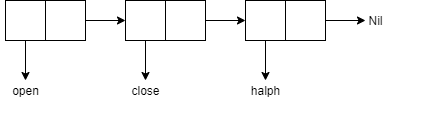
\includegraphics[scale=0.7]{task_1_1}}
\end{figure}

'((open1) (close2) (halph3))
\begin{figure}[H]
	\center{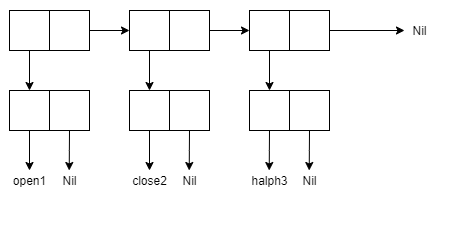
\includegraphics[scale=0.7]{task_1_2}}
\end{figure}

'((one) for all (and (me (for you))))
\begin{figure}[H]
	\center{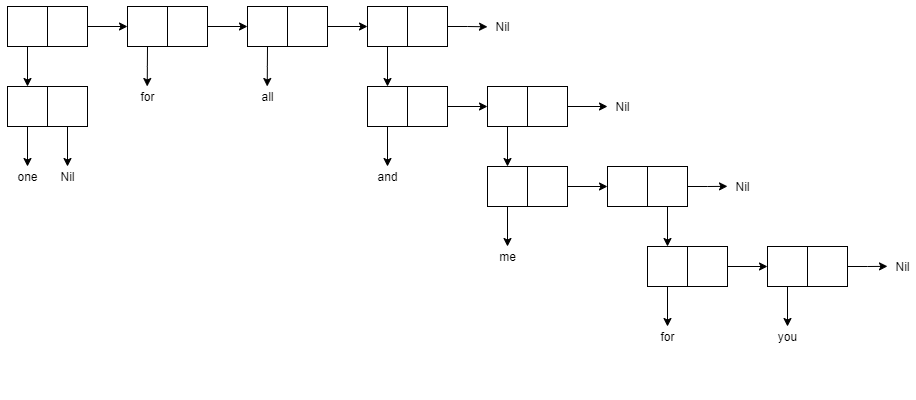
\includegraphics[scale=0.65]{task_1_3}}
\end{figure}

'((TOOL) (calll))
\begin{figure}[H]
	\center{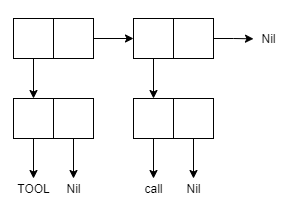
\includegraphics[scale=0.7]{task_1_4}}
\end{figure}
\newpage

'((TOOL) ((call2)) ((sell)))
\begin{figure}[H]
	\center{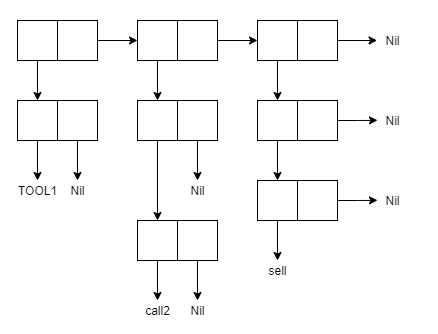
\includegraphics[scale=0.7]{task_1_5}}
\end{figure}

'(((TOOL) (call)) ((sell)))
\begin{figure}[H]
	\center{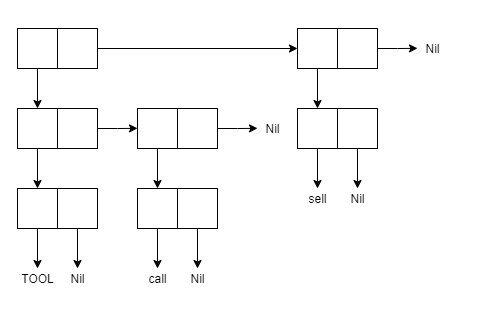
\includegraphics[scale=0.7]{task_1_6}}
\end{figure}

\section{Задание 2}
Обозначим список как <список>.
Выражения, возвращающие:
\begin{enumerate}
\item второй элемент списка --- (car (cdr '<список>));
\item третий элемент списка --- (car (cdr (cdr' <список>)));
\item четвёртый элемент списка --- (car (cdr (cdr (cdr' <список>)))).
\end{enumerate}

\section{Задание 3}
Определить результат вычисления выражения.
\begin{enumerate}
\item (caadr '((blue cube) (red pyramid))) --- red;
\item (cdar '((abc) (def) (ghi))) --- Nil;
\item (cadr '((abc) (def) (ghi))) --- (def);
\item (caddr '((abc) (def) (ghi))) --- (ghi).
\end{enumerate}
\section{Задание 4}
Определить результат вычисления выражения.
\begin{enumerate}
\item (list 'Fred 'and 'Wilma) --- (Fred and Wilma);
\item (list 'Fred '(and Wilma) --- (Fred (and Wilma));
\item (cons Nil Nil) --- (Nil);
\item (cons T Nil) --- (T);
\item (cons Nil T) --- (Nil. T);
\item (list Nil) --- (Nil);
\item (cons '(T) Nil) --- ((T));
\item (list '(one two) '(free temp)) --- ((one two) (free temp));
\item (cons 'Fred '(and Wilma)) --- (Fred and Wilma);
\item (cons 'Fred '(Wilma)) --- (Fred Wilma);
\item (list Nil Nil) --- (Nil Nil);
\item (list T Nil) --- (T Nil);
\item (list Nil T) --- (Nil T);
\item (cons T (list Nil)) --- (T Nil);
\item (list '(T) Nil) --- ((T) Nil);
\item (cons '(one two) '(free temp)) --- ((one two) free temp).
\end{enumerate}

\section{Задание 5}
Написать функцию (f ar1 ar2 ar3 ar4), возвращающую список: ((ar1 ar2) (ar3 ar4)).

Лямбда-выражение --- (lambda (ar1 ar2 ar3 ar4) (list '(ar1 ar2) '(ar3 ar4))).

Фукнция --- (defun f (ar1 ar2 ar3 ar4) (list '(ar1 ar2) '(ar3 ar4)).
\begin{figure}[H]
	\center{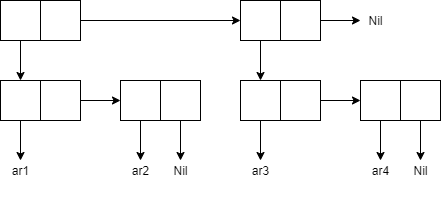
\includegraphics[scale=0.7]{task_5_1}}
\end{figure}

Написать функцию (f ar1 ar2), возвращающую ((ar1)(ar2)).

Лямбда-выражение --- (lambda (ar1 ar2) (list '(ar1) '(ar2))).

Фукнция --- (defun f (ar1 ar2) (list '(ar1) '(ar2))).
\begin{figure}[H]
	\center{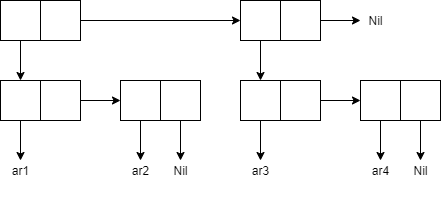
\includegraphics[scale=0.7]{task_5_1}}
\end{figure}

\newpage
Написать функцию (f ar1), возвращающую (((ar1))).

Лямбда-выражение --- (lambda (ar1) (list (list '(ar1)))).

Фукнция --- (defun f (ar1) (list (list '(ar1)))).
\begin{figure}[H]
	\center{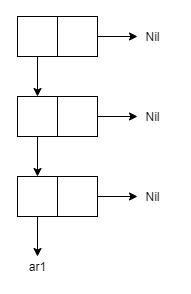
\includegraphics[scale=0.7]{task_5_3}}
\end{figure}